\section{最小二乘：近似求解}
\label{sec:ls-least-squares}
\label{sec:linear-algebra-residual-systems}
\label{sec:linear-algebra-projection-least-squares}
\label{sec:matrix-analysis-inverse-input-selection}

第~\ref{sec:ls-exact-linear-equations}节要求$\bm A\bm x=\bm b$精确成立，相容性不满足时方程无解。
观测总有误差，方程数也常多于未知数，此时不应再寻找不存在的精确解，而要在所有输入中挑选
使输出误差最小的一个。本节把“误差最小”写成可计算的平方残差目标，分别讨论普通、加权和
正则化三种目标的存在性、唯一性与选解，再给出正规方程、QR、SVD与迭代四类求解路径，
最后说明怎样按矩阵形状、数值尺度和停止准则选择方法并核验结果。灵敏度与收敛速度属于
后续扰动分析与迭代收敛章节，本节只回答目标是什么、解是否存在、怎样更新与核验。

\subsection{残差与目标}
\label{sec:ls-least-squares-objective}

给定$\bm A\in\mathbb R^{m\times d}$和观测$\bm b\in\mathbb R^m$，当不存在$\bm x$使
$\bm A\bm x=\bm b$时，改求使平方输出误差最小的输入：
\begin{equation}
 \min_{\bm x\in\mathbb R^d}\ \lVert\bm A\bm x-\bm b\rVert_2^2.
 \label{eq:linear-algebra-least-squares}
\end{equation}
这一任务称为\term{最小二乘}（least squares）。设计矩阵记号$\bm X\bm w=\bm y$只是同一问题
的回归写法，$\bm X$对应$\bm A$，系数$\bm w$对应$\bm x$，响应$\bm y$对应$\bm b$。
平方误差取欧氏长度的平方，既去掉非负平方根又保持最小点不变，也使目标成为输入的二次函数。

若$\bm b\in\operatorname{range}(\bm A)$，存在输入使残差$\bm r=\bm b-\bm A\bm x$为零，
平方残差的最小值就是$0$；此时最小二乘问题退化为第~\ref{sec:ls-exact-linear-equations}节的
相容精确方程，精确解是最小残差为零的特殊情形，而不是另一种无关的定义。以下讨论集中在
$\bm b$不可达、最小残差严格为正的一般情形。

观测可以同时有若干列。给定$\bm B\in\mathbb R^{m\times n}$，求$\bm X\in\mathbb R^{d\times n}$使
\begin{equation}
 \min_{\bm X}\ \lVert\bm A\bm X-\bm B\rVert_{\mathrm F}^2
 =\sum_{j=1}^n\lVert\bm A\bm x_j-\bm b_j\rVert_2^2,
 \label{eq:ls-multi-right-frobenius}
\end{equation}
其中$\bm b_j$、$\bm x_j$分别是$\bm B$、$\bm X$的第$j$列。Frobenius平方范数把各列残差的
平方长度相加，目标对每一列独立；因此多右端问题就是$n$个同矩阵最小二乘问题并列，分解一次
可以复用于全部列，不存在列间耦合。

不同观测的可靠程度不同，误差代价也不必相同。给定对称正定权重$\bm M\in\mathbb R^{m\times m}$，
\term{加权最小二乘}（weighted least squares）的目标为
\begin{equation}
 \min_{\bm x}\ (\bm A\bm x-\bm b)^\top\bm M(\bm A\bm x-\bm b),
 \label{eq:ls-weighted-objective}
\end{equation}
它等于在$\bm M$内积下度量残差长度，$\bm M$对角元较大的坐标误差被惩罚得更重。权重记录
各输出坐标之间的相对代价，不能与后文惩罚输入幅度的正则化参数混为一谈。若$\bm M$仅半正定，
某些坐标的误差可能被完全忽略，唯一性结论要重新检查，见~\ref{sec:ls-weighted-ls}。

\paragraph{岭回归与一般Tikhonov惩罚}

当矩阵的某些方向几乎不改变输出时，反求的系数会被放大；在数据项之外附加输入幅度的二次惩罚，
得到\term{岭回归}（ridge regression）目标
\begin{equation}
 \min_{\bm x}\ \lVert\bm A\bm x-\bm b\rVert_2^2+\lambda\lVert\bm x\rVert_2^2,
 \qquad \lambda>0.
 \label{eq:ls-ridge-objective}
\end{equation}
更一般地，惩罚可以作用在希望压小的变化量$\bm L\bm x$上，其中$\bm L\in\mathbb R^{p\times d}$
记录这种偏好，得到\term{Tikhonov正则化}（Tikhonov regularization）的一般二次形式
\scite{math-hansen2008regtools}
\begin{equation}
 \min_{\bm x}\ F_\lambda(\bm x)
 =\lVert\bm A\bm x-\bm b\rVert_2^2+\lambda\lVert\bm L\bm x\rVert_2^2,
 \qquad \lambda>0.
 \label{eq:linear-algebra-general-tikhonov}
\end{equation}
$\bm A$记录观测作用，$\bm L$记录要压小的变化，二者行数不必相同；$\bm L=\bm I$时回到岭回归。
惩罚改变的是目标本身，而不是让分解“算得出来”的实现细节：选择$\lambda$是在重新设定任务，
不能仅作为数值技巧解释。

\subsection{存在性、唯一性与选解}
\label{sec:ls-ls-existence}

先在每种目标下回答三个问题：最小点是否存在；若存在，输入是否唯一；不唯一时按什么准则
挑选代表。拟合值$\bm A\bm x$、输入$\bm x$与残差$\bm r$要分别核验，不能互相替代。

\subsubsection{普通最小二乘}
\label{sec:ls-ordinary-ls}

平方残差$\lVert\bm A\bm x-\bm b\rVert_2^2$只通过拟合值$\bm A\bm x$依赖输入：
拟合值遍历列空间$\operatorname{range}(\bm A)$，问题等价于在$\operatorname{range}(\bm A)$中
寻找离$\bm b$最近的点。第~\ref{sec:ls-subspace-nearest-points}节已经证明，有限维子空间中
到给定点的欧氏最近点存在且唯一。

因此最近拟合值$\hat{\bm b}$存在且唯一，与输入是否唯一无关。即便多个输入到达同一个
$\hat{\bm b}$，输出端的选择已经确定。最近点把$\bm b$分解为
$\bm b=\hat{\bm b}+\bm r$，其中$\hat{\bm b}\in\operatorname{range}(\bm A)$，
残差$\bm r$与整个列空间正交。

\paragraph{正交残差与正规方程}

残差与每一列正交，即对任意$\bm x$有$\bm x^\top\bm A^\top\bm r=0$，故
$\bm A^\top\bm r=\bm0$。代入$\bm r=\bm b-\bm A\hat{\bm x}$得到\term{正规方程}
（normal equations）
\begin{equation}
 \bm A^\top(\bm b-\bm A\hat{\bm x})=\bm0,
 \qquad
 \bm A^\top\bm A\hat{\bm x}=\bm A^\top\bm b.
 \label{eq:linear-algebra-normal-equations}
\end{equation}
“正规”来自法向（正交）关系，不是归一化。
图~\ref{fig:ls-least-squares-residual}把这一正交关系画成三维透视：拟合值$\bm A\hat{\bm x}$
落在列空间平面上，残差$\bm r=\bm b-\bm A\hat{\bm x}$与两条列向量都垂直。

\begin{figure}[htbp]
  \centering
  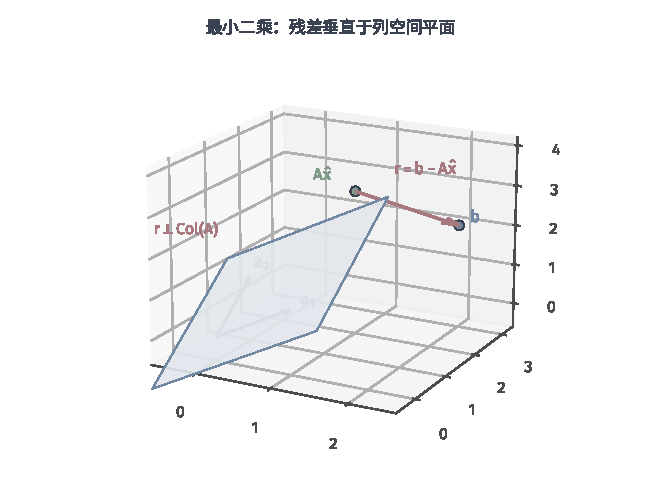
\includegraphics[width=112mm]{figures/01-mathematical-preliminaries-upper/02-linear-spaces/matplotlib/ls-least-squares-residual/ls-least-squares-residual.pdf}
  \caption{列空间平面上的最近点。$\bm A=\left[\begin{smallmatrix}1&0\\0&1\\1&1\end{smallmatrix}\right]$，
  列$\bm a_1=(1,0,1)^\top$、$\bm a_2=(0,1,1)^\top$张成浅蓝平面；$\bm b=(2,3,2)^\top$，
  最近拟合值$\bm A\hat{\bm x}=(1,2,3)^\top$，残差$\bm r=(1,1,-1)^\top$满足
  $\bm r^\top\bm a_1=\bm r^\top\bm a_2=0$。透视教学构造。}
  \label{fig:ls-least-squares-residual}
\end{figure}

正规方程不仅必要，也足以保证全局最小。对任意增量$\bm h$，
\[
 \lVert\bm A(\hat{\bm x}+\bm h)-\bm b\rVert_2^2
 =\lVert\bm A\hat{\bm x}-\bm b\rVert_2^2
 -2\bm h^\top\bm A^\top\bm r+\lVert\bm A\bm h\rVert_2^2.
\]
正规方程使中间项$\bm h^\top\bm A^\top\bm r=\bm h^\top\bm0=0$，剩下非负的
$\lVert\bm A\bm h\rVert_2^2$，故任意移动都不会减小目标。

拟合值唯一不代表输入唯一。若$\hat{\bm x}$是一个解，$\bm z\in\ker\bm A$时
$\bm A(\hat{\bm x}+\bm z)=\hat{\bm b}$不变，所以全部最优输入为
\begin{equation}
 \hat{\bm x}+\ker\bm A.
 \label{eq:ls-all-ordinary-solutions}
\end{equation}
满列秩时$\ker\bm A=\{\bm0\}$，正规矩阵$\bm A^\top\bm A$正定且可逆，唯一输入为
\begin{equation}
 \hat{\bm x}=(\bm A^\top\bm A)^{-1}\bm A^\top\bm b.
 \label{eq:linear-algebra-full-rank-least-squares}
\end{equation}
否则任意零空间增量都不改变目标，输入不唯一。

满列秩只保证系数唯一，不保证系数稳定。贯穿例（设计矩阵~\eqref{eq:linear-algebra-nearly-collinear-design}）
展示两列几乎同向时系数如何被放大。取$\bm c_1=(1,1,1)^\top$、$\bm q=(0,1,-1)^\top$，
两列为$\bm c_1$与$\bm c_1+\varepsilon\bm q$，响应$\bm y=\bm c_1+\delta\bm q$。
正规方程具体为
\[
 \begin{bmatrix}3&3\\3&3+2\varepsilon^2\end{bmatrix}\hat{\bm w}
 =\begin{bmatrix}3\\3+2\varepsilon\delta\end{bmatrix},
\]
系数矩阵行列式为$6\varepsilon^2$。$\varepsilon\neq0$时满列秩，
\begin{equation}
 \hat{\bm w}_\varepsilon
 =\begin{bmatrix}1-\delta/\varepsilon\\\delta/\varepsilon\end{bmatrix},
 \qquad\bm X_\varepsilon\hat{\bm w}_\varepsilon=\bm y,
 \label{eq:linear-algebra-nearly-collinear-least-squares}
\end{equation}
$\varepsilon=0.01$、$\delta=0.1$时系数为$(-9,10)^\top$，残差却为零。
$\varepsilon=0$时两列重合为$\bm c_1$，正交分解$\bm y=\bm c_1+\delta\bm q$的最近输出
为$\bm c_1$，残差为$\delta\bm q$（平方残差$2\delta^2$），全部系数满足$w_1+w_2=1$。
于是矩阵趋于极限时，精确拟合所需的系数发散，而极限矩阵不再能精确拟合：拟合值可以相当
稳定，表示它的两个系数却可能很大。这是近共线几何本身的结果，不是计算机造成的现象。

输入多解时需要额外准则选定代表。要求欧氏范数最小，就是去掉不改变输出的零空间分量：
把$\hat{\bm x}$分解为$(\ker\bm A)^\perp$分量与$\ker\bm A$分量，两项正交，平方范数相加，
最小值只在零空间分量为零时达到。这一选择的显式构造留给伪逆，见~\ref{sec:ls-pseudoinverse}。

\subsubsection{加权最小二乘}
\label{sec:ls-weighted-ls}

加权目标$(\bm A\bm x-\bm b)^\top\bm M(\bm A\bm x-\bm b)$中的$\bm M$对称正定。
它定义输出空间的$\bm M$内积$\langle\bm u,\bm v\rangle_{\bm M}=\bm u^\top\bm M\bm v$，
加权残差在该内积下与列空间正交。

\paragraph{白化后的普通最小二乘}

由~\ref{thm:ls-gram-factor}的配方结论，正定$\bm M$可写成$\bm M=\bm R^\top\bm R$，
其中$\bm R$可逆。令$\tilde{\bm A}=\bm R\bm A$、$\tilde{\bm b}=\bm R\bm b$，则
加权目标等于普通平方残差$\lVert\tilde{\bm A}\bm x-\tilde{\bm b}\rVert_2^2$。
这一步常称\term{白化}（whitening）：先把各坐标误差变换到同一欧氏尺度，再回到已证的
普通问题。正交条件给出加权正规方程
\begin{equation}
 \bm A^\top\bm M(\bm b-\bm A\hat{\bm x})=\bm0,
 \qquad
 \bm A^\top\bm M\bm A\,\hat{\bm x}=\bm A^\top\bm M\bm b.
 \label{eq:linear-algebra-weighted-normal-equations}
\end{equation}

白化后的最近点存在唯一，故加权拟合值$\bm A\hat{\bm x}$存在。满列秩时
$\bm A^\top\bm M\bm A$正定，输入唯一；欠定或列相关时，输入仍沿$\ker\bm A$模糊，
与普通情形同理。

若$\bm M$仅半正定，它可能忽略非零残差：例如$\bm A=\bm I$、$\bm M=\operatorname{diag}(1,0)$
时第二个拟合坐标不受目标约束，任意取值都不改变代价。被$\bm M$消去的输出方向上，
拟合值本身不再唯一，不能直接沿用正定权重的结论。

半正定$\bm M$仍给出半内积，目标在有限维输入上连续；在受约束的方向范围内取到下界，
最小点存在；不可辨认方向构成解集的仿射纤维，可在其中另取欧氏范数最小的代表。
这种选择不恢复被权重消去的信息，只是在等价解中挑一个规范代表。

多右端时若各列共用同一个$\bm M$，各列仍然独立。若不同输出坐标或不同右端列需要不同权重，
把矩阵按列向量化后，权重作用在拉长的残差向量上，列间通过权重矩阵耦合，不能再逐列独立求解。

\subsubsection{正则化最小二乘}
\label{sec:ls-regularized-ls}

一般Tikhonov目标$F_\lambda(\bm x)=\lVert\bm A\bm x-\bm b\rVert_2^2+\lambda\lVert\bm L\bm x\rVert_2^2$
同时衡量数据拟合与惩罚量。两项都非负，$\lambda>0$平衡二者；这不是普通最小二乘的近似，
而是另一个目标。

\paragraph{二次增量与正规算子}

在$\hat{\bm x}$处沿$\bm h$移动，数据项增量为
$\lVert\bm A\bm h\rVert_2^2-2\bm h^\top\bm A^\top(\bm b-\bm A\hat{\bm x})$，
惩罚项增量为$\lambda\lVert\bm L\bm h\rVert_2^2$。一阶项合并为零的条件是
\begin{equation}
 (\bm A^\top\bm A+\lambda\bm L^\top\bm L)\hat{\bm x}=\bm A^\top\bm b.
 \label{eq:ls-tikhonov-normal}
\end{equation}
系数矩阵$\bm A^\top\bm A+\lambda\bm L^\top\bm L$对称，对任意$\bm h$其二次型为
$\lVert\bm A\bm h\rVert_2^2+\lambda\lVert\bm L\bm h\rVert_2^2\geq0$。

二次型为零当且仅当$\bm A\bm h=\bm0$且$\bm L\bm h=\bm0$，即
\begin{equation}
 \ker\bm A\cap\ker\bm L=\{\bm0\}
 \label{eq:linear-algebra-tikhonov-common-nullspace}
\end{equation}
时系数矩阵正定；否则沿公共零空间方向既不改变观测也不改变惩罚，目标对该方向平坦。

正规算子对称，方程有解当且仅当右端$\bm A^\top\bm b$与其零空间正交：对公共零空间中的$\bm z$，
$\bm z^\top\bm A^\top\bm b=(\bm A\bm z)^\top\bm b=0$恒成立，故相容性自动满足，最小点存在。

$\lambda>0$时，若公共零空间为零，系数矩阵正定，增量
$\lVert\bm A\bm h\rVert_2^2+\lambda\lVert\bm L\bm h\rVert_2^2$对$\bm h\neq\bm0$严格为正，
最小点唯一。公共零空间非零时，所有最小点仍相差该空间中的向量，可另取范数最小代表，
正则化并不恢复被两者共同消去的方向。$\bm L=\bm I$时公共零空间自动为零，岭回归因而总有
唯一解；差分惩罚则未必，例如$\bm A=\bm L=[\,1\ -1\,]$时常量方向$(1,1)^\top$
仍在公共零空间中，无论$\lambda$多大都不能确定两个值的共同水平。

$\lambda=0$时目标退回普通最小二乘，唯一性由$\ker\bm A$决定；$\lambda$从正降到零是目标的
连续改变，不是同一问题的参数微调。$\lambda\to\infty$时解趋于$\ker\bm L$中的最小二乘代表，
两端的极限行为在参数选择处再用。

\subsection{直接法}
\label{sec:ls-direct-methods-ls}

直接法把系数矩阵化成可回代的因子。三种路径对应三种矩阵处境：满列秩且规模适中时形成
正规方程；要避免Gram矩阵损失尺度时用QR；秩未知、矩形且需要四个子空间时用SVD。

\subsubsection{正规方程法}
\label{sec:ls-normal-equations-method}

由~\eqref{eq:linear-algebra-normal-equations}，最小二乘解满足对称正规方程
$\bm A^\top\bm A\hat{\bm x}=\bm A^\top\bm b$。这是一个$d$阶对称方阵方程，第~\ref{sec:ls-direct-methods}节
建立的对称正定求解工具可以直接套用。

$\bm A$满列秩时$\bm A^\top\bm A$正定：$\bm x^\top\bm A^\top\bm A\bm x=\lVert\bm A\bm x\rVert_2^2$，
且$\bm A\bm x=0$只在$\bm x=0$时成立。因而正规方程有唯一解，不需要额外选解准则。

对正定$\bm A^\top\bm A$作Cholesky分解$\bm L\bm L^\top$，依次前代求$\bm L\bm z=\bm A^\top\bm b$、
回代求$\bm L^\top\hat{\bm x}=\bm z$，复用第~\ref{sec:ls-direct-methods}节的对称分解流程，
不另立新算法。加权目标对$\bm A^\top\bm M\bm A$、正则化目标对
$\bm A^\top\bm A+\lambda\bm L^\top\bm L$作同样分解，后者正定性由公共零空间条件保证。

稠密矩阵先计算$\bm A^\top\bm A$（约$md^2$次乘法），再作$d^3/3$量级的Cholesky；
多个右端复用同一分解。这一方法只需要矩阵整体可访问，适合小型满列秩问题。

形成$\bm A^\top\bm A$把小的奇异方向平方：接近零的方向被压得更小，浮点中可能直接与零
不可区分。正规方程法只在列之间明显分离、$\bm A^\top\bm A$正定余量充足时可靠；
秩亏或近秩亏时，唯一性本身已经不成立，分解成功也不给出正确选解。条件数放大的定量估计
属于扰动分析，此处只记录这一尺度损失现象。

\subsubsection{QR分解}
\label{sec:ls-qr-method}
\label{sec:linear-algebra-direct-residual}

对$\bm A$作QR分解的构造见第~\ref{sec:ls-orthogonalization-qr}节。正交矩阵保持欧氏长度，
故$\lVert\bm A\bm x-\bm b\rVert_2^2=\lVert\bm Q^\top\bm A\bm x-\bm Q^\top\bm b\rVert_2^2$，
最小点不变。这是QR适合最小二乘的根本原因：只改坐标，不改长度。

瘦QR给出$\bm A=\bm Q\bm R$，$\bm Q$列正交，$\bm R$为上三角。记
$\bm Q^\top\bm b=(\bm c_1,\bm c_2)^\top$、$\bm Q=(\bm Q_1,\bm Q_2)$，则
\[
 \lVert\bm Q\bm R\bm x-\bm b\rVert_2^2
 =\lVert\bm R\bm x-\bm c_1\rVert_2^2+\lVert\bm c_2\rVert_2^2.
\]
$\bm c_2$不依赖$\bm x$，是固定残差；可调部分只由上三角方程决定。

满列秩时$\bm R$满秩，$\bm R\hat{\bm x}=\bm c_1$上三角可直接回代，目标最小值就是
$\lVert\bm c_2\rVert_2^2$。QR不显式形成$\bm A^\top\bm A$，避免正规方程的平方尺度损失，
代价是分解本身的运算量高于Cholesky。

欠定（$m<d$）相容时，QR配合行空间表示可给出最小范数解：解落在$\operatorname{range}(\bm A^\top)$，
正交于$\ker\bm A$。完整的最小范数构造在伪逆处给出，此处只说明QR同样服务于这一选解。

带列主元的QR按接近独立的顺序排列列，使接近零的对角元集中到尾部，从而暴露数值秩。
秩的阈值与噪声尺度有关，见~\ref{sec:ls-method-selection}。

秩亏时取前$r$个主元列回代得到一个基本解，自由方向补零；它是一个合法最优解，但未必
最小范数。核验时同时检查输出残差$\bm b-\bm A\hat{\bm x}$与最优性残差
$\bm A^\top(\bm b-\bm A\hat{\bm x})$，并在需要最小范数时核对$\hat{\bm x}$是否正交于
$\ker\bm A$。

\subsubsection{SVD分解}
\label{sec:ls-svd}

QR只处理满列秩或秩揭示的情形；秩未知、矩形矩阵需要同时给出非零方向、零方向、四个子空间
和稳定选解时，使用奇异值分解。它的存在性不能假设：下面先用实对称谱引理从单位球极值
直接构造，这也是全卷首次建立谱定理，后续球面极值、低秩逼近与矩阵函数都复用这一结论。

对任意$\bm A\in\mathbb R^{m\times d}$，希望找到两组正交方向，使$\bm A$在其间只作独立
伸缩。这需要先证明\term{谱定理}（spectral theorem）：对称矩阵能在正交基下对角化。

\begin{lemma}[实对称谱引理]
\label{thm:ls-real-symmetric-spectral}
\label{thm:matrix-analysis-symmetric-spectral-theorem}
\label{sec:ch06-triangular-spectrum}
设$\bm S\in\mathbb R^{d\times d}$满足$\bm S=\bm S^\top$。存在正交矩阵$\bm Q$与实对角
$\Lambda=\operatorname{diag}(\lambda_1,\dots,\lambda_d)$，使
\begin{equation}
 \bm S=\bm Q\Lambda\bm Q^\top,
 \qquad \bm S\bm q_i=\lambda_i\bm q_i.
 \label{eq:matrix-analysis-symmetric-eigendecomposition}
\end{equation}
对任意$\bm x=\sum_i c_i\bm q_i$，二次型展开为
\begin{equation}
 \bm x^\top\bm S\bm x=\sum_{i=1}^d\lambda_i c_i^2.
 \label{eq:matrix-analysis-quadratic-spectral-form}
\end{equation}
\end{lemma}

\begin{proof}
单位球面$\{\bm x:\lVert\bm x\rVert_2=1\}$是$\mathbb R^d$中的闭有界集，二次型
$q(\bm x)=\bm x^\top\bm S\bm x$连续，由~\ref{thm:ls-extreme-value}在球上取到最大值
$\lambda_1$，记最大点为$\bm q_1$，$\lVert\bm q_1\rVert_2=1$。实对称保证
$\lambda_1=\bm q_1^\top\bm S\bm q_1$是实数。

任取与$\bm q_1$正交的$\bm h$，实数$t$很小时$\bm q_1+t\bm h$归一化后仍在球上，
故其二次型不超过$\lambda_1$倍范数平方。展开：
\[
 \lambda_1+2t\bm h^\top\bm S\bm q_1+t^2\bm h^\top\bm S\bm h
 \leq\lambda_1(1+t^2\lVert\bm h\rVert_2^2).
\]
两边减去$\lambda_1$，$t$的一阶项$2t\bm h^\top\bm S\bm q_1$必须对正负$t$同时不破坏
不等式，因而只能为零，即$\bm h^\top\bm S\bm q_1=0$。对所有$\bm h\perp\bm q_1$成立，
说明$\bm S\bm q_1$没有正交分量，只能平行于$\bm q_1$，即$\bm S\bm q_1=\lambda_1\bm q_1$。
全程只用有限代数增量，不引入复特征多项式。

对$\bm h\perp\bm q_1$，$\bm q_1^\top\bm S\bm h=(\bm S\bm q_1)^\top\bm h
=\lambda_1\bm q_1^\top\bm h=0$，故$\bm S$把$\bm q_1^\perp$映到自身，限制仍是对称矩阵。
在$d-1$维正交补上重复同一极值构造，得到$\bm q_2,\lambda_2$；归纳到一维即得正交列
$\bm q_1,\dots,\bm q_d$与实特征值$\lambda_i$。代入$\bm x=\sum_i c_i\bm q_i$交叉项为零，
便得到谱展开式。这一证明只依赖球的紧性与对称配对，是实情形的完整谱定理；复Hermitian
情形的共轭转置推广在矩阵函数章再给。
\end{proof}

令$\bm S=\bm A^\top\bm A$，它对称且半正定：$\bm x^\top\bm A^\top\bm A\bm x
=\lVert\bm A\bm x\rVert_2^2\geq0$。由谱引理，存在标准正交的$\bm v_i$使
$\bm A^\top\bm A\bm v_i=\lambda_i\bm v_i$，且$\lambda_i\geq0$。记正特征值为
$\sigma_i^2=\lambda_i>0$（$i=1,\dots,r$），$\sigma_i>0$，按降序排列；其余$\bm v_j$满足
$\bm A^\top\bm A\bm v_j=0$，因而$\bm A\bm v_j=0$。

对$\sigma_i>0$定义$\bm u_i=\bm A\bm v_i/\sigma_i$。它们标准正交：
\[
 \bm u_i^\top\bm u_j
 =\frac{\bm v_i^\top\bm A^\top\bm A\bm v_j}{\sigma_i\sigma_j}
 =\frac{\sigma_i^2\delta_{ij}}{\sigma_i\sigma_j}=\delta_{ij}.
\]
且$\bm A\bm v_i=\sigma_i\bm u_i$。

$\bm v_{r+1},\dots,\bm v_d$是$\ker\bm A$的标准正交基；把$\bm u_1,\dots,\bm u_r$扩充为
$\mathbb R^m$的标准正交基，多余方向落在$\operatorname{range}(\bm A)^\perp$。于是
$\bm A$写成秩一矩阵之和
\begin{equation}
 \bm A=\sum_{i=1}^r\sigma_i\bm u_i\bm v_i^\top.
 \label{eq:matrix-analysis-svd-rank-one-sum}
\end{equation}
其中$r=\operatorname{rank}\bm A$，非零奇异值个数就是秩。

\begin{theorem}[SVD的存在与构造]
\label{thm:ls-svd-existence}
对任意$\bm A\in\mathbb R^{m\times d}$，上述构造给出正交$\bm U\in\mathbb R^{m\times m}$、
$\bm V\in\mathbb R^{d\times d}$与对角$\Sigma\in\mathbb R^{m\times d}$，非负对角元
$\sigma_i$使$\bm A=\bm U\Sigma\bm V^\top$。
\end{theorem}

\begin{definition}[奇异值分解]
\label{def:matrix-analysis-svd}
称
\begin{equation}
 \bm A=\bm U\Sigma\bm V^\top
 \label{eq:matrix-analysis-svd}
\end{equation}
为\term{奇异值分解}（singular value decomposition, SVD），非负对角元$\sigma_i$为
\term{奇异值}（singular value），$\bm u_i$、$\bm v_i$分别为左、右\term{奇异向量}
（singular vector）。
\end{definition}

图~\ref{fig:ls-svd-construction}把这一构造拆成三步：先形成对称$\bm A^\top\bm A$，
再由谱引理正交对角化取特征值，最后开方得奇异值、并由$\bm u_i=\bm A\bm v_i/\sigma_i$
得左奇异向量。

\begin{figure*}[htbp]
  \centering
  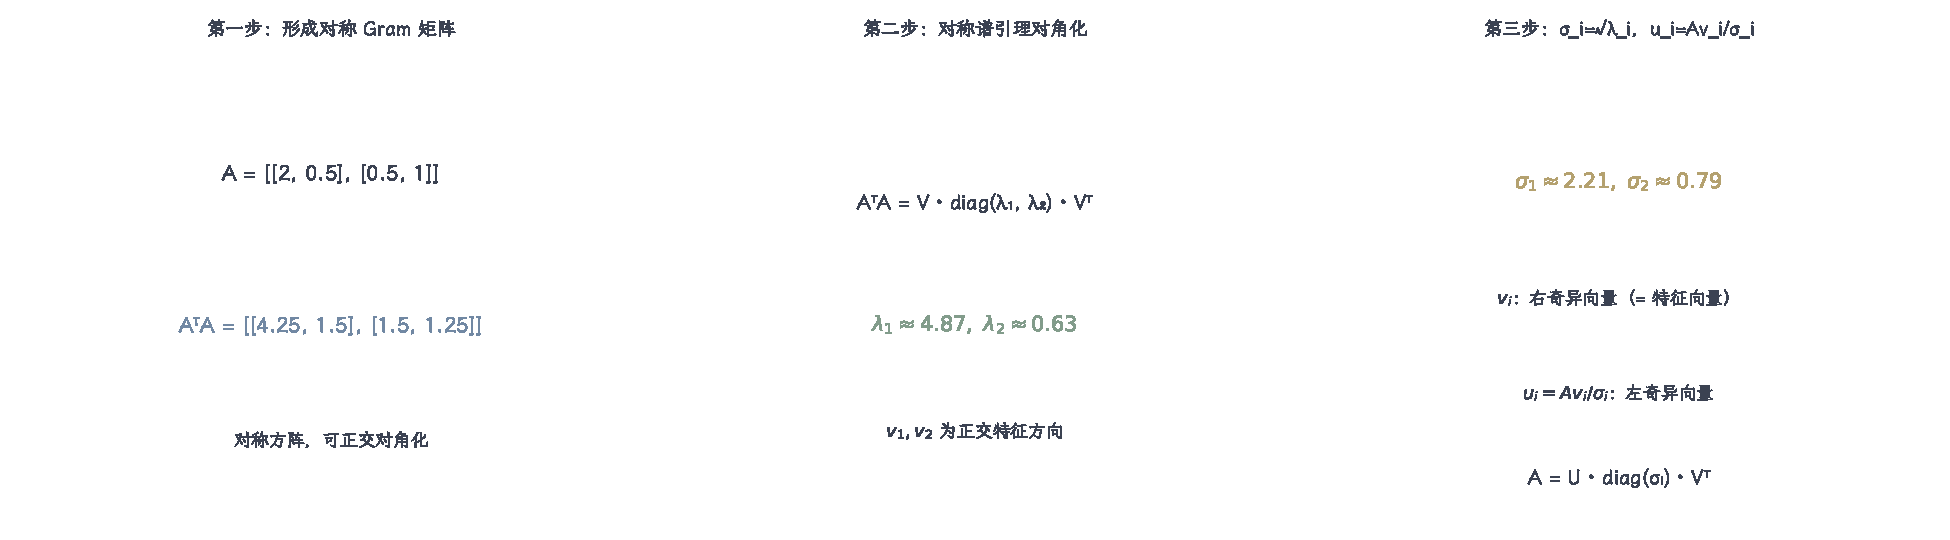
\includegraphics[width=168.998mm]{figures/01-mathematical-preliminaries-upper/02-linear-spaces/matplotlib/ls-svd-construction/ls-svd-construction.pdf}
  \caption{SVD 构造三部曲。以$\bm A=\left[\begin{smallmatrix}2&0.5\\0.5&1\end{smallmatrix}\right]$为例：
  (1)形成$\bm A^\top\bm A=\left[\begin{smallmatrix}4.25&1.5\\1.5&1.25\end{smallmatrix}\right]$；
  (2)对称谱引理对角化，特征值$\lambda_1\approx4.87,\lambda_2\approx0.63$；
  (3)$\sigma_i=\sqrt{\lambda_i}\approx2.21,0.79$，右奇异向量$\bm v_i$即特征向量，
  左奇异向量$\bm u_i=\bm A\bm v_i/\sigma_i$。解析式教学构造。}
  \label{fig:ls-svd-construction}
\end{figure*}

图~\ref{fig:matrix-analysis-svd-geometry}使用二维旋转矩阵
$\bm R(\theta)=
\left[\begin{smallmatrix}\cos\theta&-\sin\theta\\\sin\theta&\cos\theta\end{smallmatrix}\right]$
构造一个左右方向不同的变换，两侧采用相同比例便于比较伸缩量。

\begin{figure*}[htbp]
  \centering
  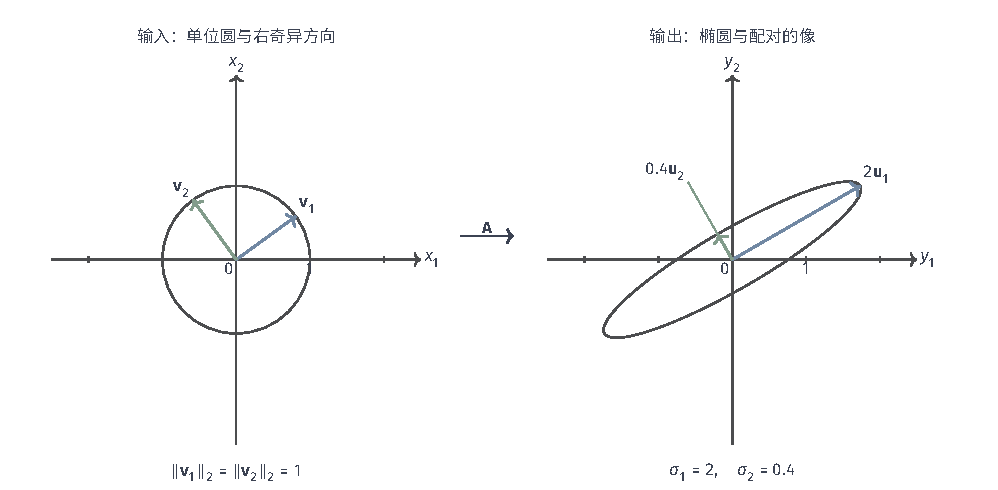
\includegraphics[width=168.998mm]{figures/01-mathematical-preliminaries-upper/02-linear-spaces/tikz/matrix-analysis-svd-geometry/figure.pdf}
  \caption{矩阵$\bm A=\bm R(\pi/6)\operatorname{diag}(2,0.4)\bm R(\pi/5)^\top$
  将单位圆变为椭圆。蓝、绿分别对应两个奇异方向；同色箭头在左侧标出$\bm v_i$，
  在右侧标出其像$\sigma_i\bm u_i$。两侧坐标比例相同。奇异值决定长度变化，左右方向可以不同，
  因而这不是沿特征方向的同空间缩放。图为教学构造。}
  \label{fig:matrix-analysis-svd-geometry}
\end{figure*}

与这一“单位圆变椭圆”的输入侧视角互补，图~\ref{fig:ls-svd-ellipse-action}从行图像与
列图像两侧看最小二乘解：左图两条方程直线交于$\hat{\bm x}=(1,1)^\top$，残差二次型的
水平集是以它为中心的同心椭圆；右图$\bm b$恰落在列空间内，残差为零。

\begin{figure*}[htbp]
  \centering
  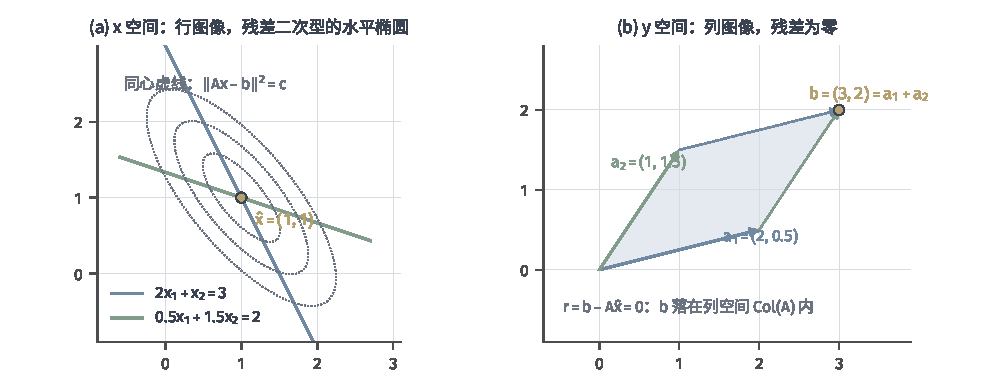
\includegraphics[width=168.998mm]{figures/01-mathematical-preliminaries-upper/02-linear-spaces/matplotlib/ls-svd-ellipse-action/ls-svd-ellipse-action.pdf}
  \caption{最小二乘解的行图像与列图像。$\bm A=\left[\begin{smallmatrix}2&1\\0.5&1.5\end{smallmatrix}\right]$、
  $\bm b=(3,2)^\top$，$\bm A\hat{\bm x}=\bm b$恰有解$\hat{\bm x}=(1,1)^\top$。左：两条方程直线
  交于$\hat{\bm x}$，灰色点线为残差平方$f(\bm x)=\lVert\bm A\bm x-\bm b\rVert_2^2$的水平集，
  中心即交点；右：列$\bm a_1=(2,0.5)^\top$、$\bm a_2=(1,1.5)^\top$张成列空间，
  $\bm b=\bm a_1+\bm a_2$落在其中，残差为零。解析式教学构造。}
  \label{fig:ls-svd-ellipse-action}
\end{figure*}

$\sigma_i$相同时，对应子空间内的任意标准正交旋转仍给出分解，故$\bm U,\bm V$不唯一；
奇异值本身由$\bm A$唯一确定。零奇异值对应的方向不参与伸缩。

数值实现先以Householder双边约化把矩阵变成上双对角形（复用~\ref{sec:ls-orthogonalization-qr}
的反射工具），再用隐式QR位移迭代得到对角元；直接对$\bm A^\top\bm A$求特征值会重蹈
平方尺度损失，故实现始终作用在原矩阵上。

以贯穿例的二维约化看清两个尺度。把设计的输出限制到$\operatorname{span}\{\bm c_1,\bm q\}$，
用$\bm c_1/\sqrt3$、$\bm q/\sqrt2$作正交坐标，再将全部输出统一除以$\sqrt3$，
得到二维表示
\begin{equation}
 \bm X_{\widetilde\varepsilon}
 =\begin{bmatrix}1&1\\0&\widetilde\varepsilon\end{bmatrix},
 \qquad \widetilde\varepsilon=\sqrt{2/3}\,\varepsilon.
 \label{eq:matrix-analysis-nearly-collinear-design}
\end{equation}
这一统一缩放把奇异值除以$\sqrt3$，不改变它们的比值。二维Gram矩阵为
$\bm G_{\widetilde\varepsilon}
=\begin{bmatrix}1&1\\1&1+\widetilde\varepsilon^2\end{bmatrix}$，
其两个特征值由二次方程得到
\begin{equation}
 \lambda_\pm
 =\frac{2+\widetilde\varepsilon^2
          \mathbin{\pm}\sqrt{4+\widetilde\varepsilon^4}}{2},
 \label{eq:matrix-analysis-nearly-collinear-gram-eigenvalues}
\end{equation}
对$\widetilde\varepsilon>0$，$\sigma_\pm=\sqrt{\lambda_\pm}$；
$\widetilde\varepsilon\to0$时$\sigma_{\max}\to\sqrt2$、
$\sigma_{\min}\sim\widetilde\varepsilon/\sqrt2$。大方向近似为两个系数一起变化，
小方向近似为两个系数相消。这一推导只用于理解谱；为计算小奇异值不应显式形成Gram矩阵，
也不宜用相近两数相减求$\lambda_-$，定量原因留给扰动章节。

完整SVD给出$\bm U,\bm V$全正交基；只需要前$k$个奇异方向时可计算薄分解，省去尾部。
稠密完整分解的运算量高于QR，但其明示全部奇异值、四个子空间与最小二乘选解，是秩未知
矩形矩阵的通用工具。

\subsubsection{伪逆与全部最优解}
\label{sec:ls-pseudoinverse}

先看一个欠定小例。$\bm A=[2\ 0]$把$(x_1,x_2)^\top$映成$2x_1$，取$\bm b=(3)$：
方程$2x_1=3$的全部解为$(3/2,t)^\top$，$t$任意，输出只由$x_1$决定。
范数平方$(3/2)^2+t^2$在$t=0$时最小，代表点$(3/2,0)^\top$——它自动落在
$\operatorname{range}(\bm A^\top)$方向上、把零空间分量压为零。伪逆就是把“全部解中
范数最小者”写成一个矩阵的规则：本例$\bm A^\dagger=(1/2,0)^\top$，
$\bm A^\dagger\bm b=(3/2,0)^\top$。下面用SVD把这一规则推广到任意秩。

在$\bm v_i$方向上$\bm A$以$\sigma_i$伸缩到$\bm u_i$，反向自然除以$\sigma_i$：
$\bm u_i\mapsto\bm v_i/\sigma_i$。把$\bm b$按$\bm u_i$展开，可恢复分量
$(\bm u_i^\top\bm b)/\sigma_i$配给$\bm v_i$；落在$\operatorname{range}(\bm A)^\perp$的
分量没有原像，直接丢弃；零方向$\bm v_{r+1},\dots$上$\bm A$没有输出，反向不定义。
小$\sigma_i$在正向作用中压缩，反求时把该分量放大，这是伪逆对弱方向敏感的来源，定量
放大分析属扰动章节。

\begin{definition}[Moore--Penrose伪逆]
\label{def:matrix-analysis-pseudoinverse}
在两端标准内积下，\term{Moore--Penrose伪逆}（Moore--Penrose pseudoinverse）先把
输出正交投影到$\operatorname{range}(\bm A)$，再在$(\ker\bm A)^\perp$上反演：
\[
 \bm A^\dagger=(\bm A|_{(\ker\bm A)^\perp})^{-1}P_{\operatorname{range}(\bm A)}.
\]
用~\ref{thm:ls-svd-existence}的SVD写出即
\begin{equation}
 \bm A^\dagger=\sum_{i=1}^r\frac{1}{\sigma_i}\bm v_i\bm u_i^\top,
 \label{eq:matrix-analysis-pseudoinverse}
\end{equation}
它在$\operatorname{range}(\bm A)^\perp$上取零；$\bm A=\bm0$时定义$\bm A^\dagger=\bm0$。
普通逆是伪逆在可逆方阵上的特殊情形。
\end{definition}

\begin{theorem}[最小二乘与最小范数]
\label{thm:matrix-analysis-pseudoinverse-minimum-norm}
给定$\bm A\in\mathbb R^{m\times d}$和$\bm b\in\mathbb R^m$，全部最小二乘解为
$\bm A^\dagger\bm b+\ker\bm A$，其中$\bm A^\dagger\bm b$是唯一的最小欧氏范数解；
方程相容时它就是全部精确解中的最小范数者。
\begin{proof}
记$P_R$为到$\operatorname{range}\bm A$的正交投影。把
$\bm b=P_R\bm b+\bm b_\perp$（$\bm b_\perp\perp\operatorname{range}\bm A$）、
$\bm x=\bm x_\perp+\bm x_N$（$\bm x_N\in\ker\bm A$）正交分解，则
\[
 \lVert\bm A\bm x-\bm b\rVert_2^2
 =\lVert\bm A\bm x_\perp-P_R\bm b\rVert_2^2+\lVert\bm b_\perp\rVert_2^2.
\]
第二项不能由输入改变；第一项在且仅在$\bm x_\perp$等于投影反演
$(\bm A|_{(\ker\bm A)^\perp})^{-1}P_R\bm b$，也就是$\bm A^\dagger\bm b$时为零。
故全部最优输入为$\bm A^\dagger\bm b+\bm x_N$。两项正交，
$\lVert\bm x\rVert_2^2=\lVert\bm A^\dagger\bm b\rVert_2^2+\lVert\bm x_N\rVert_2^2$，
最小值仅在$\bm x_N=0$时达到。相容时$\bm b_\perp=0$，同一证明适用。
\end{proof}
\end{theorem}

\paragraph{Penrose条件的逐项验证}

由SVD和式直接相乘逐项核对四条：
\begin{enumerate}
 \item $\bm A\bm A^\dagger\bm A=\bm A$；
 \item $\bm A^\dagger\bm A\bm A^\dagger=\bm A^\dagger$；
 \item $(\bm A\bm A^\dagger)^\top=\bm A\bm A^\dagger$；
 \item $(\bm A^\dagger\bm A)^\top=\bm A^\dagger\bm A$。
\end{enumerate}
前两项保证在可反演部分上一致，后两条说明
$\bm A\bm A^\dagger$是到$\operatorname{range}(\bm A)$的正交投影、
$\bm A^\dagger\bm A$是到$(\ker\bm A)^\perp$的正交投影。

满足同样四条的矩阵唯一：若$\bm G$也满足，则$\bm A\bm G=P_R$、$\bm G\bm A=P_{(\ker\bm A)^\perp}$，
于是$\bm G=\bm G\bm A\bm G=P_{(\ker\bm A)^\perp}\bm A^\dagger=\bm A^\dagger$。
故伪逆不由SVD写法决定，是矩阵本身的性质。

$\bm A\bm A^\dagger=\sum_i\bm u_i\bm u_i^\top=P_{\operatorname{range}(\bm A)}$，
$\bm A^\dagger\bm A=\sum_i\bm v_i\bm v_i^\top=P_{(\ker\bm A)^\perp}$；
$\operatorname{range}(\bm A^\dagger)=(\ker\bm A)^\perp$，
$\ker(\bm A^\dagger)=\operatorname{range}(\bm A)^\perp$。四个子空间分属输入端与输出端，
与伴随的正交补关系一致。

例如$\bm A=\begin{smallmatrix}1&1\\0&0\end{smallmatrix}$、$\bm b=(2,1)^\top$，
可达输出只有第二坐标为零的$(2,0)^\top$，残差$(0,1)^\top$无法消除；原像直线
$x_1+x_2=2$上平方范数为$2+2t^2$，伪逆选择$t=0$得到$(1,1)^\top$。伪逆没有使
原本无解的方程突然可解，也没有恢复被$\bm A$消去的信息。

\begin{figure*}[htbp]
  \centering
  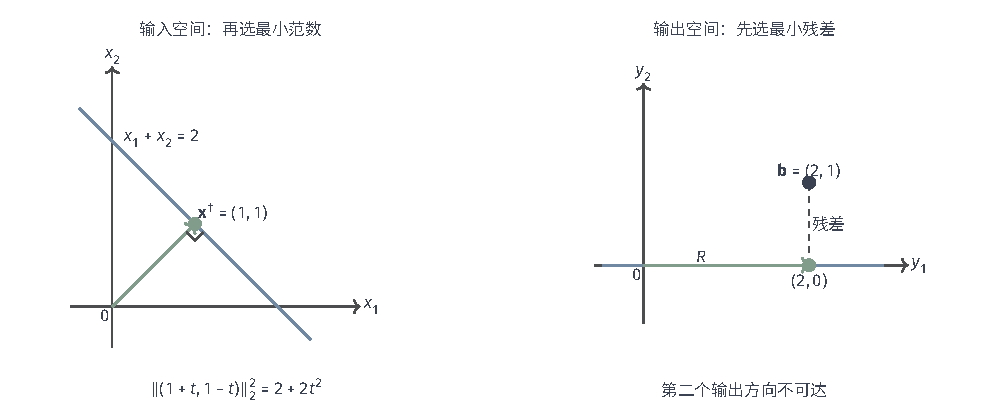
\includegraphics[width=168.998mm]{figures/01-mathematical-preliminaries-upper/02-linear-spaces/tikz/matrix-analysis-pseudoinverse-selections/figure.pdf}
  \caption{伪逆的两次选择。右图先在可达输出中选择离$\bm b=(2,1)^\top$最近的
  $(2,0)^\top$；左图再在整条原像直线$x_1+x_2=2$上选择最靠近原点的$(1,1)^\top$。
  两图属于不同空间，各自等比例绘制。}
  \label{fig:matrix-analysis-pseudoinverse-selections}
\end{figure*}

全部最优输入为
\begin{equation}
 \hat{\bm x}=\bm A^\dagger\bm b+\bm z,
 \qquad \bm z\in\ker\bm A.
 \label{eq:ls-all-pseudoinverse-solutions}
\end{equation}
由证明中的正交分解，$\bm z=0$时范数最小。这就完成了~\ref{sec:ls-ordinary-ls}节
承诺的选解构造。

满列秩时$\bm A^\dagger=(\bm A^\top\bm A)^{-1}\bm A^\top$；满行秩时
$\bm A^\dagger=\bm A^\top(\bm A\bm A^\top)^{-1}$，用于相容欠定系统的最小范数恢复。
任意秩直接用SVD和式，不要套用只在满秩成立的逆公式；伪逆对矩阵不连续（非零标量
$\varepsilon$的伪逆为$1/\varepsilon$，零标量的伪逆为零），秩改变是必须检查的边界。

对~\eqref{eq:ls-multi-right-frobenius}，矩阵最优解为$\bm A^\dagger\bm B$，各列独立取伪逆；
最小范数选解逐列一致，不存在列间耦合。

\subsubsection{加权与正则化的求解}
\label{sec:ls-weighted-regularized-solve}

由$\bm M=\bm R^\top\bm R$把加权问题变成普通最小二乘：$\tilde{\bm A}=\bm R\bm A$、
$\tilde{\bm b}=\bm R\bm b$后，对$\tilde{\bm A}$使用前述QR或SVD，结果代回原变量即得
加权解，不必重造适合$\bm M$的分解。

Tikhonov目标写成普通最小二乘的\term{增广最小二乘}（augmented least squares）形式：
\begin{equation}
 \begin{bmatrix}\bm A\\ \sqrt{\lambda}\,\bm L\end{bmatrix}\bm x
 \approx\begin{bmatrix}\bm b\\ \bm0\end{bmatrix}.
 \label{eq:ls-augmented-system}
\end{equation}
增广矩阵的正规方程正是~\eqref{eq:ls-tikhonov-normal}，故所有普通最小二乘工具原样复用，
不引入新求解器。

若已有$\bm A$的SVD$\bm A=\bm U\Sigma\bm V^\top$且$\bm L=\bm I$，岭解在奇异坐标中为
\begin{equation}
 \hat{\bm x}_\lambda=\sum_{i=1}^r\frac{\sigma_i}{\sigma_i^2+\lambda}
 \bm v_i(\bm u_i^\top\bm b),
 \label{eq:matrix-analysis-ridge-filter-factor}
\end{equation}
每个方向被$\sigma_i/(\sigma_i^2+\lambda)$收缩；小$\sigma_i$方向的放大被压回。
这一收缩改变了解的偏差，其定量放大与偏差分析属于扰动章节，此处只记录表达式。

白化或增广得到的是变换后坐标，必须代回$\bm x$并在原目标中核验：普通项
$\lVert\bm A\hat{\bm x}-\bm b\rVert_2^2$、惩罚项$\lambda\lVert\bm L\hat{\bm x}\rVert_2^2$
与正规方程残差三者分别检查，不能只报变换空间中的残差。

半正定$\bm M$或公共零空间非零时，增广系统在不可辨认方向上仍无唯一解，需另取最小范数
代表；此时不要指望$\lambda$或权重本身恢复被消去的方向。

\subsection{迭代法}
\label{sec:ls-least-squares-iterative}

矩阵只以“给向量返回乘积”的形式给出、或分解填充远超原矩阵时，不构造因子，用序列逼近。
本节只给更新、执行条件与核验量；误差随步数下降的速率证明属于迭代收敛章节。

\subsubsection{Landweber迭代}
\label{sec:ls-landweber}
\label{sec:linear-algebra-gradient-residual}

残差$\bm r=\bm b-\bm A\bm w$沿输出空间；把它搬回输入端的方向是$\bm A^\top\bm r$，
它正是正规方程残差$\bm A^\top\bm b-\bm A^\top\bm A\bm w$。这一伴随作用不需要显式矩阵。

沿$\bm g=\bm A^\top(\bm A\bm w-\bm b)$移动一步，目标增量的一阶项为负；要保证每步不反弹，
步长须使最大伸缩方向的更新倍率绝对值小于$1$，即$0<\eta<2/\lVert\bm A\rVert_2^2$，
其中$\lVert\bm A\rVert_2=\sigma_1$为最大奇异值，由~\ref{thm:ls-svd-existence}的谱定义。

\paragraph{Landweber更新和步长}
\begin{equation}
 \bm w^{(t+1)}=\bm w^{(t)}+\eta\bm A^\top(\bm b-\bm A\bm w^{(t)}),
 \qquad 0<\eta<\frac{2}{\sigma_1^2}.
 \label{eq:ch06-least-squares-gradient-update}
\end{equation}
每步一次$\bm A$作用和一次$\bm A^\top$作用，不形成$\bm A^\top\bm A$。

$\ker\bm A$中的分量不被$\bm A^\top$读取，迭代始终保留初值在$\ker\bm A$中的部分；
零初值收敛到最小范数解，非零初值则保留其零空间分量。收敛证明与极限形式留待收敛章节。

每步核验两个量：输出残差$\bm r^{(t)}=\bm b-\bm A\bm w^{(t)}$与最优性残差
$\bm g^{(t)}=\bm A^\top\bm r^{(t)}$；前者衡量拟合，后者衡量正规方程。每步代价为两次
矩阵向量乘积加若干内积，存储只需要几个向量。

\subsubsection{CGLS迭代}
\label{sec:ls-cgls}

CGLS把共轭梯度法用于正规方程$\bm A^\top\bm A\bm w=\bm A^\top\bm b$，但只在
$\operatorname{range}(\bm A^\top)$内展开，正规方程的CG框架复用第~\ref{sec:ls-krylov-methods}节，
不重复证明有限步终止与正交性。

搜索方向与残差只通过$\bm A\bm p$、$\bm A^\top\bm r$两次乘积更新，从不显式形成
$\bm A^\top\bm A$，因而避免正规算子的平方尺度损失，也不要求矩阵整体存储；只要能给出
正向与伴随乘积，CGLS即可执行。

\paragraph{CGLS的残差和方向更新}

取$\bm w^{(0)}$，$\bm r^{(0)}=\bm b-\bm A\bm w^{(0)}$，$\bm g^{(0)}=\bm A^\top\bm r^{(0)}$，
$\bm p^{(0)}=\bm g^{(0)}$；每步按CG系数更新
\[
 \alpha=\frac{(\bm g^{(t)})^\top\bm g^{(t)}}{(\bm p^{(t)})^\top\bm A^\top\bm A\bm p^{(t)}},
 \quad
 \bm w^{(t+1)}=\bm w^{(t)}+\alpha\bm p^{(t)},
 \quad
 \bm r^{(t+1)}=\bm r^{(t)}-\alpha\bm A\bm p^{(t)},
\]
\[
 \bm g^{(t+1)}=\bm A^\top\bm r^{(t+1)},\qquad
 \beta=\frac{(\bm g^{(t+1)})^\top\bm g^{(t+1)}}{(\bm g^{(t)})^\top\bm g^{(t)}},
 \qquad
 \bm p^{(t+1)}=\bm g^{(t+1)}+\beta\bm p^{(t)}.
\]
分母中的$\bm A^\top\bm A\bm p$以两次乘积实现。

CG只在$\operatorname{range}(\bm A^\top)$内展开搜索空间，零初值且$\ker\bm A$非零时，
迭代自然停在该子空间，给出最小范数解；非零初值保留其$\ker\bm A$分量，不会被算法擦除，
与Landweber相同。要最小范数代表就从$\bm w^{(0)}=\bm0$起步。

以$\lVert\bm g^{(t)}\rVert_2$达到容限为主停止量，同时重算原始残差$\bm r^{(t)}$核验，
不用递推残差直接判定。每步两次乘积、三个方向向量，存储随步数不线性增长。

\subsubsection{LSQR迭代}
\label{sec:ls-lsqr}

CGLS作用在正规算子$\bm A^\top\bm A$上，继承其尺度；LSQR直接在原最小二乘问题上工作，
交替从输出端和输入端投影，适合正规算子病态而原问题本身可解的情形。它同样只调用
$\bm A$与$\bm A^\top$，不显式形成平方矩阵。

从$\bm u_1=\bm b/\lVert\bm b\rVert_2$出发，反复交替用$\bm A^\top$把当前输出方向
映回输入端、再用$\bm A$映回输出端，每步把新方向正交化并归一化，逐步把$\bm A$投影成
下双对角小矩阵；全过程只调用$\bm A$与$\bm A^\top$，不显式形成正规算子。

$k$步后基中系数$\bm z_k$满足等价的小规模最小二乘
\[
 \min_{\bm z_k}\ \lVert\beta_1\bm e_1-\bar{\bm B}_k\bm z_k\rVert_2,
\]
双对角小矩阵维数仅$k$，可用QR直接求解，避免在原空间做大分解。

$\bm w^{(k)}$由输入端基$\bm v_j$按$\bm z_k$的系数线性组合恢复；解不必显式累加全部基，
可用递推公式边走边更新，存储量由实现控制。

零初值在$\operatorname{range}(\bm A^\top)$内逼近最小范数解；秩亏时停止步与容限共同
决定截取哪些方向，过早停止起隐式正则化作用，这一现象的定量分析属扰动章节。

LSQR直接掌握原始残差$\bm b-\bm A\bm w^{(k)}$，核验时重算该残差与$\bm A^\top$投影，
不依赖递推；每步两次乘积加一个双对角小问题求解，基存储随$k$增加，实际使用常配合重启。

\subsubsection{加权与正则化的迭代}
\label{sec:ls-iterative-reuse}

加权问题先白化：正向$\tilde{\bm A}\bm x=\bm R\bm A\bm x$，伴随为$\bm A^\top\bm R^\top$；
对白化后的普通问题跑上述迭代，代价只是把乘积换成加权作用。

正则化增广算子$\begin{bmatrix}\bm A\\\sqrt{\lambda}\bm L\end{bmatrix}$的正向作用拼接
$\bm A\bm x$与$\sqrt{\lambda}\bm L\bm x$，伴随作用拼接$\bm A^\top\bm u$与
$\sqrt{\lambda}\bm L^\top\bm v$，迭代法照用，不需要显式构造增广矩阵。

Landweber、CGLS、LSQR都不依赖具体矩阵元素，只要求可计算正向与伴随乘积。因此把加权
或正则化看成一个新算子后，更新格式、停止量与存储结构原样复用，加权、正则化是换算子，
不是换算法。

停止判定必须回到原目标：加权残差$\lVert\bm M^{1/2}(\bm A\hat{\bm x}-\bm b)\rVert_2$、
正则化目标$F_\lambda(\hat{\bm x})$与各自最优性残差分别检查，不以变换空间残差代替，
否则会把变换误差误当成原目标误差。

\subsection{方法选择与结果核验}
\label{sec:ls-method-selection}

满列秩、小型、矩阵整体可访问：正规方程Cholesky最省；满列秩但近共线：QR避免平方损失；
秩未知、矩形、需要子空间与选解：SVD。数值秩不是绝对零：把奇异值与数据误差、机器精度
按整体尺度比较，远小于$\sigma_1$且低于噪声水平的方向判为零，阈值随整体尺度缩放，
不设脱离尺度的绝对数。需要最小范数选解时优先SVD伪逆或零初值迭代。

决策先看矩阵如何提供：能整体存入且可分解的中小规模问题走直接法；只能逐向量调用乘积、
矩阵无法整体访问的走迭代法；分解填充远超原矩阵的稀疏问题同样选迭代，预条件本身的构造
与作用成本要计入总代价，不能只比迭代步数。

任何解都分别核验：输出残差$\bm r=\bm b-\bm A\hat{\bm x}$是否达到任务容限；正规方程残差
$\bm g=\bm A^\top\bm r$是否为零；最小范数要求下$\hat{\bm x}$是否正交于$\ker\bm A$。
迭代停止以$\lVert\bm g\rVert$与$\lVert\bm r\rVert$共同为准，递推残差适时用高精度重算。

\paragraph{参数选择、差异原则与残差容限}

正则化参数$\lambda$不由拟合好坏单独决定。\term{差异原则}（discrepancy principle）给定
允许残差$\delta$，求解约束问题
\begin{equation}
 \min_{\lVert\bm A\bm x-\bm b\rVert_2\leq\delta}\ \lVert\bm L\bm x\rVert_2^2,
 \label{eq:ls-discrepancy-constrained}
\end{equation}
其等价的$\lambda$问题是$\min F_\lambda$。记$R(\lambda)=\lVert\bm A\bm x_\lambda-\bm b\rVert_2^2$、
$P(\lambda)=\lVert\bm L\bm x_\lambda\rVert_2^2$。对$0<\lambda_1<\lambda_2$，由$\bm x_{\lambda_1}$
最小化$F_{\lambda_1}$得$R_1+\lambda_1P_1\leq R_2+\lambda_1P_2$，即
$R_1-R_2\leq\lambda_1(P_2-P_1)$；由$\bm x_{\lambda_2}$最小化$F_{\lambda_2}$得
$R_2+\lambda_2P_2\leq R_1+\lambda_2P_1$，即$R_1-R_2\geq\lambda_2(P_2-P_1)$。两式联立
\[
 \lambda_2(P_2-P_1)\leq R_1-R_2\leq\lambda_1(P_2-P_1).
\]
因$\lambda_2>\lambda_1\geq0$，左端不超过右端只可能$P_2-P_1\leq0$，即$P_2\leq P_1$；
进而$R_1-R_2\leq\lambda_1(P_2-P_1)\leq0$，即$R_1\leq R_2$。故惩罚项$P(\lambda)$单调
不增、残差$R(\lambda)$单调不减：$\lambda$越大越压小$\bm L\bm x$，代价是拟合残差上升。
连续性来自正定增广正规方程$(\bm A^\top\bm A+\lambda\bm L^\top\bm L)\bm x_\lambda
=\bm A^\top\bm b$的解对$\lambda$的连续依赖：$\lambda>0$时系数矩阵正定，其逆与
$\bm x_\lambda$都是$\lambda$的有理函数，$R(\lambda)$、$P(\lambda)$随之连续。
记$R(0)$为$\lambda=0$处普通最小二乘的最小可达残差，$R(\infty)$为$\lambda\to\infty$、
$\bm x$被限制在$\ker\bm L$内时的残差（$\bm L=\bm I$时$\bm x\to\bm 0$，
$R(\infty)=\lVert\bm b\rVert_2^2$）。于是：$\delta<R(0)$时无可行解；
$R(0)\leq\delta<R(\infty)$时由单调性与连续性存在满足$R(\lambda)=\delta$的$\lambda$，
按$R(\lambda)$随$\lambda$上升的方向二分搜索；$\delta\geq R(\infty)$时约束不起作用，
取尽可能大的惩罚，解退化为$\ker\bm L$上的最小二乘。

当$R(0)\leq\delta<R(\infty)$，约束取等号$R(\lambda)=\delta$，对应$\lambda>0$的惩罚问题；
二者解相同，$\lambda$是约束乘子。$\delta\geq R(\infty)$时约束松弛，惩罚取最大。
这一对应也说明：选择$\delta$等价于设定可接受的观测误差，参数不是
自由调节的数值旋钮。图~\ref{fig:ls-regularization-bias-variance}用固定的二元例子
把这一单调折中画出来：$\lambda$增大时残差$R(\lambda)$上升、参数范数$P(\lambda)$下降。

\begin{figure*}[htbp]
  \centering
  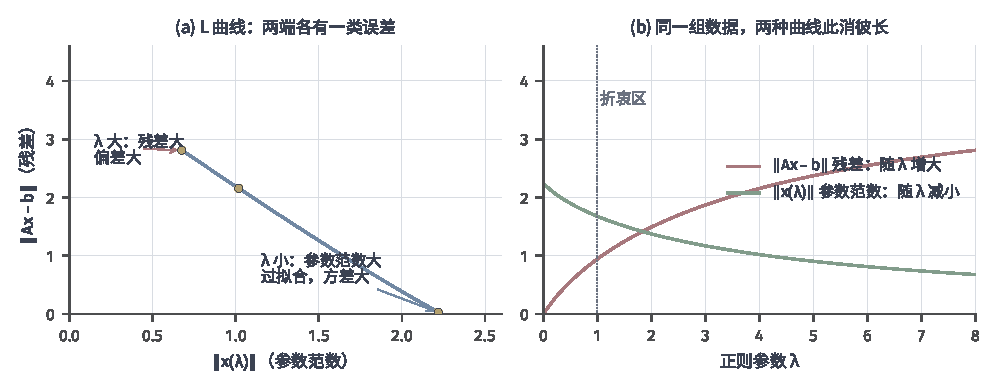
\includegraphics[width=168.998mm]{figures/01-mathematical-preliminaries-upper/02-linear-spaces/matplotlib/ls-regularization-bias-variance/ls-regularization-bias-variance.pdf}
  \caption{正则化的偏差—方差折中。$\bm A=\operatorname{diag}(2,1)$、$\bm b=(4,1)^\top$，
  岭解$\bm x(\lambda)=(8/(4+\lambda),1/(1+\lambda))^\top$。左：L曲线——横轴参数范数
  $\lVert\bm x(\lambda)\rVert$、纵轴残差$\lVert\bm A\bm x-\bm b\rVert$；右端（$\lambda$小）
  拟合准但参数大，左端（$\lambda$大）参数小但残差大。右：残差随$\lambda$上升、
  参数范数随$\lambda$下降，灰色虚线为折衷区。固定复算，无采样。}
  \label{fig:ls-regularization-bias-variance}
\end{figure*}

\section{二次优化}
\label{sec:ls-quadratic-optimization}

最小二乘目标本身是二次的；把“平方长度”推广到一般对称二次型，加上无约束、球面约束、
子空间约束与线性等式约束，得到一族可完全用代数配方和~\ref{sec:ls-svd}建立的谱定理
解决的优化问题。本节不使用微积分：所有最优性条件都由平方增量非负和正交关系得到。

\subsection{目标与约束}
\label{sec:ls-quadratic-goal}

一般二次目标写成（\term{二次型}，quadratic form）
\begin{equation}
 f(\bm x)=\frac12\bm x^\top\bm M\bm x+\bm c^\top\bm x,
 \label{eq:ls-general-quadratic}
\end{equation}
其中$\bm M$不必对称。反对称部分$\frac12(\bm M-\bm M^\top)$满足
$\bm x^\top(\bm M-\bm M^\top)\bm x=0$，故二次型只由对称部分
$\bm S=\frac12(\bm M+\bm M^\top)$决定，以下一律取$\bm S=\bm S^\top$。

无约束问题为$\min_{\bm x\in\mathbb R^d}f(\bm x)$；带线性等式约束为
\begin{equation}
 \min\ f(\bm x)\quad\text{s.t.}\quad \bm C\bm x=\bm d,
 \label{eq:ls-equality-constrained}
\end{equation}
$\bm C\in\mathbb R^{p\times d}$。可行性先于优化：$\bm C\bm x=\bm d$必须相容。

不含线性项时目标为$\bm x^\top\bm S\bm x$（可取$1/2$因子）。齐次性使目标在尺度缩放
下按平方变化，因而自然约束在单位球面$\lVert\bm x\rVert_2=1$、闭球
$\lVert\bm x\rVert_2\leq1$或某个子空间中；球面消除尺度自由度，只比较方向。

长度由$\bm B\succ0$度量时，约束为$\bm x^\top\bm B\bm x=1$，即\term{广义球面}；
它把加权长度固定，仍只优化方向。

\subsection{存在性与唯一性}
\label{sec:ls-quadratic-existence}

先判定目标在给定集合上是否有下界、极小点是否存在、是否唯一，再谈求解。

\subsubsection{无约束问题}
\label{sec:ls-unconstrained-existence}

先看三个二元例子区分目标形状：$f_1(x,y)=x^2+2y^2$恒正、原点是唯一谷底；
$f_2(x,y)=x^2$沿$y$轴整条等高，$f_2=0$取遍$(0,y)$，最小值集合是一条直线；
$f_3(x,y)=x^2-y^2$在原点一方向上谷、另一方向上脊，是鞍点。
图~\ref{fig:ls-quadratic-level-sets}把三类水平集并置：正定是同心椭圆，半正定退化为
平行直线槽，不定是双曲线。它们的差别只在$\bm S$的惯性（正、负、零特征值个数）。

\begin{figure*}[htbp]
  \centering
  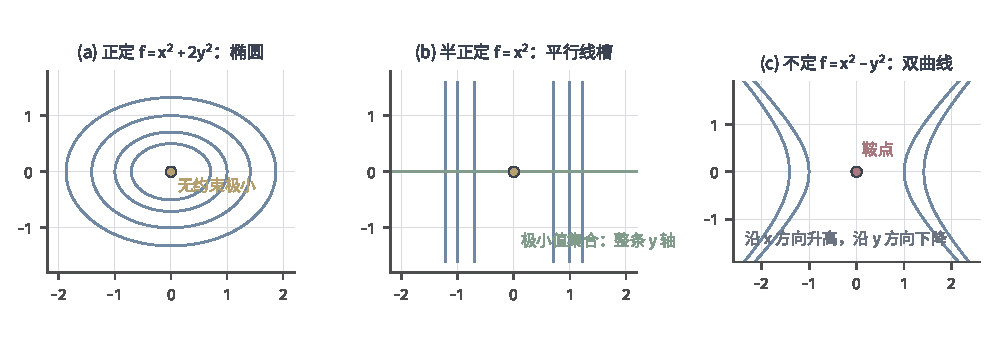
\includegraphics[width=168.998mm]{figures/01-mathematical-preliminaries-upper/02-linear-spaces/matplotlib/ls-quadratic-level-sets/ls-quadratic-level-sets.pdf}
  \caption{二次型水平集的三种情形。(a)正定$f=x^2+2y^2$：四层同心椭圆，黄点为唯一极小
  $(0,0)$；(b)半正定$f=x^2$：水平集退化为竖直线，绿线是极小值集合——整条$y$轴；
  (c)不定$f=x^2-y^2$：双曲线，红点为鞍点，沿$x$方向是谷、沿$y$方向是脊。
  解析式直接求值。}
  \label{fig:ls-quadratic-level-sets}
\end{figure*}

由谱引理~\ref{thm:ls-real-symmetric-spectral}，$\bm S$的正交谱展开把任意
$\bm x=\sum_i c_i\bm q_i$代入得
$f(\bm x)=\frac12\sum_i\lambda_i c_i^2+\sum_i c_i\bm c^\top\bm q_i$，每个方向独立。

若$\bm S$有负特征值$\lambda_j<0$，沿$\bm q_j$取$\bm x=t\bm q_j$，二次项
$\frac12\lambda_jt^2$按$t^2$趋向$-\infty$，线性项只按$t$一次增长，$|t|$足够大时
$t^2$项主导，目标无下界，不存在最小值。因此不定矩阵上的驻点不能当作最小点。

$\bm S\succeq0$时每个$\lambda_i\geq0$，二次项非负且沿正特征方向增长。零特征方向
$\lambda_j=0$上二次项为常数，目标只保留该方向的线性项；这些方向是否把目标拉向$-\infty$，
必须单独检查，不能因为二次项非负就认定有下界。

零方向$\bm q_j$上若有线性分量$\bm c^\top\bm q_j\neq0$，取$\bm x=t\bm q_j$，目标中的
线性项$t\,\bm c^\top\bm q_j$在$t\to-\infty$时趋向$-\infty$。故有下界的必要条件是
$\bm c\perp\ker\bm S$，由对称算子$\operatorname{range}\bm S=(\ker\bm S)^\perp$，
即$\bm c\in\operatorname{range}\bm S$。这也是正规方程$\bm S\bm x=-\bm c$相容的条件。

$\bm S\succ0$时所有$\lambda_i>0$，目标沿每个方向严格增长，唯一极小点。
$\bm S\succeq0$且$\bm c\in\operatorname{range}\bm S$时，正规方程相容，极小点存在
但沿$\ker\bm S$方向平坦，解集为仿射空间$\bm x_*+\ker\bm S$；不另加范数最小准则则
答案不唯一。

满足$\bm S\bm x+\bm c=0$的点只是驻点（最优性方程成立）。$\bm S$不定时，沿正特征方向
移动目标上升、沿负特征方向下降，驻点两侧一升一降，是鞍点而非最小点。不能把“方程成立”
当作“最小”，必须同时检查$\bm S$没有负方向；驻点条件只给出候选，不给出优劣判定。

\paragraph{惯性、合同判据与有界性}

$\bm S$的\term{惯性}（inertia）指正、负、零特征值的个数三元组$(n_+,n_-,n_0)$，由
谱引理唯一确定。目标有无下界恰由$n_-$判定：$n_->0$即存在负方向，目标无下界；
$n_-=0$（半正定）时二次项非负，目标有下界。合同变换（用可逆$\bm P$作
$\bm P^\top\bm S\bm P$）保持三个计数不变，故无需真的算出特征值，也可由对称消元记录
主元符号判断有界性。

\subsubsection{球面与子空间约束}
\label{sec:ls-sphere-existence}
\label{sec:linear-algebra-homogeneous-estimation}
\label{sec:linear-algebra-constrained-estimation}

单位球面$\{\bm x:\lVert\bm x\rVert_2=1\}$在有限维中是闭有界集，连续函数
$\bm x^\top\bm S\bm x$由~\ref{thm:ls-extreme-value}在球上同时取到最大值和最小值，
与$\bm S$是否正定无关；不定矩阵的两个极值分居零两侧。这一存在性不依赖方向是否可解，
先保证极值点存在，再讨论它落在哪个谱方向。

\paragraph{尺度消去与Rayleigh商}

齐次目标$\bm x^\top\bm S\bm x$在$\bm x\neq0$上按平方缩放变化，直接优化会被长度主导。
把长度约掉，方向评价写成\term{Rayleigh商}（Rayleigh quotient）
\begin{definition}[Rayleigh商]
\label{def:matrix-analysis-rayleigh-quotient}
\begin{equation}
 R_{\bm S}(\bm x)=\frac{\bm x^\top\bm S\bm x}{\bm x^\top\bm x},
 \label{eq:matrix-analysis-rayleigh-quotient}
\end{equation}
\end{definition}
它在$\bm x$缩放任意非零倍时不变，因此求$R_{\bm S}$的极值等价于在单位球面上求
$\bm x^\top\bm S\bm x$的极值，长度自由度被完全消去。

把$\bm x=\sum_i c_i\bm q_i$代入，分母$\sum_i c_i^2=1$（球面），
$R_{\bm S}(\bm x)=\sum_i\lambda_i c_i^2$是特征值以权重$c_i^2$（和为$1$）作的加权平均，
故落在$[\lambda_{\min},\lambda_{\max}]$内；令权重全给$\lambda_1$得最大值、全给
$\lambda_d$得最小值，且分别在$\bm q_1$、$\bm q_d$上取等。

$\lambda_i=\lambda_j$时，这两个特征向量的任意标准正交组合仍是该特征值的特征方向，
张成的子空间中每个单位向量都给出同一个极值商。故极值值唯一，达到它的方向一般不唯一；
仅当目标特征值单重时，方向才只差一个符号。图~\ref{fig:ls-sphere-constrained-extremum}
用一个二元对称矩阵把这一相切关系画出：极值椭圆恰在特征方向处与单位圆相切。

\begin{figure}[htbp]
  \centering
  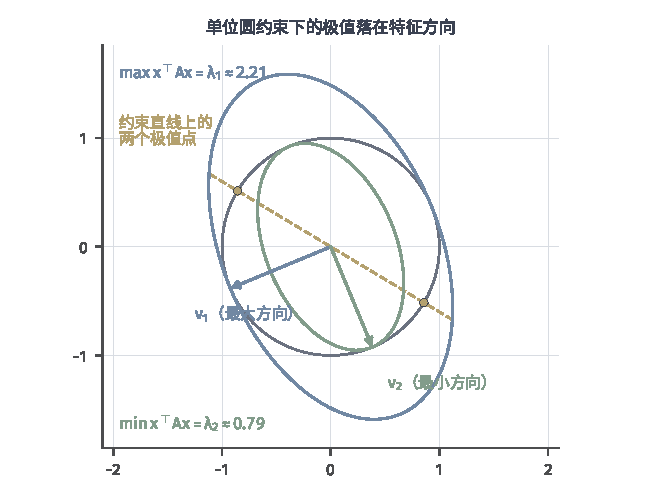
\includegraphics[width=112mm]{figures/01-mathematical-preliminaries-upper/02-linear-spaces/matplotlib/ls-sphere-constrained-extremum/ls-sphere-constrained-extremum.pdf}
  \caption{单位圆约束下的极值落在特征方向。$\bm S=\left[\begin{smallmatrix}2&0.5\\0.5&1\end{smallmatrix}\right]$，
  灰圆为$\lVert\bm x\rVert=1$。蓝椭圆$\bm x^\top\bm S\bm x=\lambda_1\approx2.21$在
  $\pm\bm v_1$处与单位圆相切（最大值），绿椭圆$=\lambda_2\approx0.79$在$\pm\bm v_2$处
  相切（最小值）；黄色虚线为子空间约束直线，其上黄点是该约束下的两个极值。
  $\lambda_{1,2}=(3\pm\sqrt2)/2$。固定复算。}
  \label{fig:ls-sphere-constrained-extremum}
\end{figure}

闭球$\lVert\bm x\rVert\leq1$是有界闭集，极值同样存在。$\bm S\succeq0$时最小值$0$
在内部$\bm x=0$取到，方向问题因此被迫放到边界；$\bm S$不定时最小值为负，落在
边界球面上，内部只含$\bm x=0$这个平凡点。所以“非零方向估计”必须主动固定单位长度，
否则齐次目标会把平凡解$\bm x=0$当作答案。

\paragraph{子空间约束下的同一问题}

限制在子空间$\mathcal W$中，问题仍是$\min_{\bm x\in\mathcal W}R_{\bm S}(\bm x)$，
由$\mathcal W$上的限制谱决定，是特征值交错与广义特征问题的入口。典型应用是
\term{齐次最小二乘}（homogeneous least squares）：模型写成$\bm A\bm h\approx\bm0$，
直接最小化$\lVert\bm A\bm h\rVert_2^2$总会接受平凡解$\bm h=\bm0$，必须先固定非零尺度：
\begin{equation}
 \min_{\lVert\bm h\rVert_2=1}\ \lVert\bm A\bm h\rVert_2^2
 =\min_{\lVert\bm h\rVert_2=1}\bm h^\top\bm A^\top\bm A\bm h.
 \label{eq:linear-algebra-homogeneous-least-squares}
\end{equation}
由Rayleigh--Ritz，最小值为$\bm A^\top\bm A$的最小特征值，最优$\bm h$是对应单位特征向量，
即最弱右奇异方向。$\bm A$有非零零空间时最小值为零，任一单位零空间向量都达到最优；
特别地$m<d$时不能只看紧致SVD列出的正奇异值而漏掉右零空间。最小特征值单重时方向只差
符号，重数更大则比例也不足以唯一确定。例如$\bm A=[\,1\ -2\,]$只要求$h_1=2h_2$，
单位解为$\pm(2,1)^\top/\sqrt5$，两个符号表示同一个实比例。

\subsubsection{线性等式约束}
\label{sec:ls-equality-existence}

优化只在可行集上进行，先判定$\bm C\bm x=\bm d$相容（$\bm d\in\operatorname{range}\bm C$）；
不相容时没有可行点，问题无解，谈不上优化。相容但$\bm C$的行线性相关时，多余方程是
独立方程的线性组合，不改变可行集，求解前可先去冗余，缩小约束规模。

取一个特解$\bm x_0$满足$\bm C\bm x_0=\bm d$，令$\mathcal N=\ker\bm C$，其标准正交基
排成矩阵$\bm N$。于是$\bm C(\bm x-\bm x_0)=\bm0$当且仅当$\bm x-\bm x_0\in\mathcal N$，
全部可行点参数化为$\bm x=\bm x_0+\bm N\bm z$，$\bm z$自由；可行方向就是$\mathcal N$。

把参数化代入$f(\bm x)=\frac12\bm x^\top\bm S\bm x+\bm c^\top\bm x$，二次项化为
$\bm z^\top(\bm N^\top\bm S\bm N)\bm z$，一次项化为
$\bm z^\top\bm N^\top(\bm c+\bm S\bm x_0)$，常数项与$\bm z$无关；问题化为
$\bm N^\top\bm S\bm N$在$\bm z$上的无约束二次问题，只在可行方向内检查曲率。

$\bm N^\top\bm S\bm N$在$\mathcal N$上正定，即$\bm z\neq0$时
$\bm z^\top\bm N^\top\bm S\bm N\bm z>0$；此时约化目标严格凸，唯一可行极小点，
代回参数化即得唯一$\hat{\bm x}$。

$\bm N^\top\bm S\bm N\succeq0$时，约化线性项$\bm N^\top(\bm c+\bm S\bm x_0)$
必须落在其值域内；若它沿某个零方向有分量，沿该方向移动时二次项不变而线性项下降，
目标无下界。条件满足时解集为$\bm x_*+\ker(\bm N^\top\bm S\bm N)$的仿射空间。

约化二次型在$\mathcal N$上有负方向，则沿该方向取$\bm x=\bm x_0+t\bm N\bm z$，
二次项按$t^2$趋向$-\infty$，约束问题无下界，与无约束情形同理。

\subsection{直接求解}
\label{sec:ls-quadratic-direct}

\subsubsection{无约束二次最小化}
\label{sec:ls-unconstrained-solve}

$\bm S\succ0$时把二次项配成完全平方：取$\bm x_*$满足$\bm S\bm x_*=-\bm c$，则
\[
 f(\bm x)-f(\bm x_*)=\frac12(\bm x-\bm x_*)^\top\bm S(\bm x-\bm x_*),
\]
右端因$\bm S$正定而非负，且只在$\bm x=\bm x_*$时为零。故$\bm S\bm x_*=-\bm c$给出
唯一最优线性方程，最小化问题归结为解这个正定对称方程。

$\bm S$正定，复用~\ref{sec:ls-direct-methods}的Cholesky分解$\bm S=\bm L\bm L^\top$，
先前代解$\bm L\bm y=-\bm c$，再回代解$\bm L^\top\bm x_*=\bm y$，避免形成逆矩阵。
分解与右端多重时可共享；这一路线与最小二乘正规方程用的是同一条正定对称求解流程。

$\bm S\succeq0$且$\bm c\in\operatorname{range}\bm S$时，$\bm S\bm x_*=-\bm c$相容。
由配方，任一解$\bm x_*$都是极小点；沿$\ker\bm S$移动二次项不变，全部解为
$\bm x_*+\ker\bm S$的仿射空间。不另加范数最小准则则答案不唯一，选代表的方法与普通
最小二乘的零空间选择相同。

核验两点：最优性方程$\bm S\hat{\bm x}+\bm c=0$成立；且对任意$\bm x$，增量
$\frac12(\bm x-\hat{\bm x})^\top\bm S(\bm x-\hat{\bm x})\geq0$非负。若增量沿某方向
为负，则该点不是最小点；方程成立只说明候选，符号检查才给出最小性。

\subsubsection{球面与子空间极值}
\label{sec:ls-sphere-solve}

\begin{theorem}[Rayleigh--Ritz]
\label{thm:matrix-analysis-rayleigh-ritz}
\label{eq:matrix-analysis-rayleigh-ritz}
设$\bm S$谱分解$\bm S=\sum_i\lambda_i\bm q_i\bm q_i^\top$，
$\lambda_1\geq\cdots\geq\lambda_d$，则
\begin{equation}
 \max_{\bm x\neq0}R_{\bm S}(\bm x)=\lambda_1\ \text{（在}\bm q_1\text{取到）},\qquad
 \min_{\bm x\neq0}R_{\bm S}(\bm x)=\lambda_d\ \text{（在}\bm q_d\text{取到）}.
\end{equation}
\end{theorem}
\begin{proof}
由谱展开$R_{\bm S}(\bm x)$是特征值的加权平均，故介于$\lambda_d$与$\lambda_1$之间；
取$\bm x=\bm q_1$、$\bm x=\bm q_d$时分别等于$\lambda_1$、$\lambda_d$，夹逼得端点取等。
\end{proof}

单方向极值只给$\lambda_1$与$\lambda_d$。要刻画中间的$\lambda_k$，取任意$k$维子空间
$\mathcal V$：它与$\operatorname{span}\{\bm q_k,\dots,\bm q_d\}$（维数$d-k+1$）的
维数之和$k+(d-k+1)=d+1>d$，故必有非零交点，交点处的Rayleigh商不大于$\lambda_k$。
换一个$d-k+1$维子空间与$\operatorname{span}\{\bm q_1,\dots,\bm q_k\}$同理相交。
这一维数交点关系是Courant--Fischer最小最大原理的几何来源。

\paragraph{Courant--Fischer的上下界与取等}

\begin{theorem}[Courant--Fischer]
\label{thm:matrix-analysis-courant-fischer}
\label{eq:matrix-analysis-courant-fischer}
\begin{equation}
 \lambda_k=\max_{\dim\mathcal V=k}\ \min_{\bm x\in\mathcal V,\bm x\neq0}R_{\bm S}(\bm x)
 =\min_{\dim\mathcal W=d-k+1}\ \max_{\bm x\in\mathcal W,\bm x\neq0}R_{\bm S}(\bm x).
\end{equation}
\end{theorem}
\begin{proof}
取$\mathcal V=\operatorname{span}\{\bm q_1,\dots,\bm q_k\}$，其中任意单位向量的
Rayleigh商不小于$\lambda_k$，给出下界；任一$k$维子空间与$\operatorname{span}\{\bm q_k,\dots,\bm q_d\}$
相交，交点处商不大于$\lambda_k$，给出上界。另一式由正交补同理得到。
\end{proof}
它不要求预先知道特征向量，为只需要第$k$个极值的子空间搜索提供了存在性表述。

\paragraph{正交列约束下的迹极值}

给定$k$个标准正交列$\bm V\in\mathbb R^{d\times k}$（$\bm V^\top\bm V=\bm I_k$），
\begin{theorem}[迹极值]
\label{thm:matrix-analysis-trace-minimum}
\label{eq:matrix-analysis-trace-minimum}
\begin{equation}
 \min_{\bm V^\top\bm V=\bm I_k}\operatorname{tr}(\bm V^\top\bm S\bm V)
 =\sum_{i=d-k+1}^d\lambda_i,
 \qquad
 \max_{\bm V^\top\bm V=\bm I_k}\operatorname{tr}(\bm V^\top\bm S\bm V)
 =\sum_{i=1}^k\lambda_i,
\end{equation}
\end{theorem}
\begin{proof}
由谱展开$\operatorname{tr}(\bm V^\top\bm S\bm V)=\sum_i\lambda_i\lVert\bm q_i^\top\bm V\rVert_2^2$，
权重$\lVert\bm q_i^\top\bm V\rVert_2^2$非负且总和为$k$；把权重配给最小的$k$个
$\lambda_i$得最小值，配给最大的$k$个得最大值，对应特征向量张成达到取等。
\end{proof}
最小值由$k$个最小特征向量张成，最大值由$k$个最大特征向量张成；这是后续正交拟合与
低秩方向提取的代数基础。

广义约束$\bm x^\top\bm B\bm x=1$、$\bm B\succ0$，先由Cholesky
$\bm B=\bm R^\top\bm R$令$\bm z=\bm R\bm x$，则约束化为$\lVert\bm z\rVert_2=1$，
目标$\bm x^\top\bm S\bm x$化为$\bm z^\top\bm R^{-\top}\bm S\bm R^{-1}\bm z$，成为
普通对称矩阵$\bm R^{-\top}\bm S\bm R^{-1}$的Rayleigh商，可直接用单方向极值结论。

\paragraph{广义特征问题与方向恢复}

\begin{definition}[广义特征值]
\label{def:matrix-analysis-generalized-eigenvalue}
白化后的对称问题等价于\term{广义特征问题}
\begin{equation}
 \bm S\bm v=\mu\bm B\bm v,
 \label{eq:matrix-analysis-generalized-eigenproblem}
\end{equation}
\end{definition}
白化后普通特征向量$\bm z$恢复原方向$\bm v=\bm R^{-1}\bm z$；广义极值即$\mu$的最大、
最小值，方向按此恢复。不要直接对$\bm B^{-1}\bm S$（一般非对称）求特征，其特征值可能为
复数而失去极值意义。

\subsubsection{等式约束二次最小化}
\label{sec:ls-equality-solve}

由可行点参数化$\bm x=\bm x_0+\bm N\bm z$，把约束消去后，目标化为$\bm z$上的无约束
二次问题，正规方程为
$(\bm N^\top\bm S\bm N)\bm z=-\bm N^\top(\bm c+\bm S\bm x_0)$；解出$\bm z$后按
$\bm x=\bm x_0+\bm N\bm z$拼回原变量。这一路线先把可行性编入参数化，求解时不必再
显式处理约束。

约化矩阵$\bm N^\top\bm S\bm N$正定即按无约束流程Cholesky求解，得到唯一$\hat{\bm z}$；
半正定则按值域条件解相容方程，在全部最小点中选代表。约化矩阵维数等于$\ker\bm C$的
维数，通常小于原问题规模。

对任意可行方向$\bm\delta$（$\bm C\bm\delta=0$），目标沿$\bm\delta$的一阶变化为
$\bm\delta^\top(\bm S\bm x+\bm c)$，最优性要求它为零。这说明$\bm S\bm x+\bm c$正交于
$\ker\bm C$，由正交补关系落在$\operatorname{range}(\bm C^\top)$，故存在乘子$\bm\mu$
使$\bm S\bm x+\bm c=\bm C^\top\bm\mu$；$\bm\mu$衡量约束方向上的平衡量。

\paragraph{KKT系统的分块构造}

联立约束$\bm C\bm x=\bm d$与最优性$\bm S\bm x+\bm c=\bm C^\top\bm\mu$，得到
\term{KKT条件}（KKT conditions）分块系统
\begin{equation}
 \begin{bmatrix}\bm S&\bm C^\top\\ \bm C&\bm0\end{bmatrix}
 \begin{bmatrix}\bm x\\ \bm\mu\end{bmatrix}
 =\begin{bmatrix}-\bm c\\ \bm d\end{bmatrix}.
 \label{eq:ls-kkt-system}
\end{equation}
它同时编码可行性（第二块行）与最优性（第一块行），由正交关系推出，不需要微分记号。

对分块系统可先消元（把$\bm\mu$从第一行解出代回），或对分块矩阵作适当分解直接求解，
同时得到$\bm x$与$\bm\mu$。$\bm\mu$只是伴随约束的对偶量，不改变原目标值，核验时
主要保证$\bm x$满足原目标与约束。

$\ker\bm C\cap\ker\bm S=\{\bm0\}$时$\bm\mu$唯一；约束冗余（$\bm C$行相关）时
$\operatorname{range}\bm C^\top$维数小于行数，$\bm\mu$可加$\ker\bm C^\top$中的量而
不改变方程，乘子不唯一，但可行方向正定时原变量$\bm x$仍可唯一。

分别核验：可行性$\bm C\hat{\bm x}=\bm d$；最优性$\bm S\hat{\bm x}+\bm c\in\operatorname{range}(\bm C^\top)$，
即对所有$\bm\delta\in\ker\bm C$有$\bm\delta^\top(\bm S\hat{\bm x}+\bm c)=0$。只满足约束
或只满足方程都不是合格最小点，二者缺一不可。

\subsection{迭代求解}
\label{sec:ls-quadratic-iterative}

直接法需要分解矩阵；只给矩阵作用时用迭代逼近谱方向或正定极小点，收敛速度证明留待
迭代收敛章节。

$\bm S\succ0$的无约束问题$\bm S\bm x=-\bm c$本身就是正定对称线性方程，直接复用
~\ref{sec:ls-krylov-methods}的共轭梯度法：每步只调用$\bm S$对向量的乘积，不形成分解，
更新格式、有限步终止与停止核验在该处建立，此处不重述。

求最大特征方向时反复$\bm v\leftarrow\bm S\bm v/\lVert\bm S\bm v\rVert_2$：每次作用把
最大特征值方向按$\lambda_1$放大，其余方向按比值$\lambda_i/\lambda_1$相对缩小，归一化
后方向逐次偏向$\bm q_1$。相邻特征值分离越快，比值越小，方向提取越直接；分离程度决定
收敛快慢，定量速率留待迭代收敛章节。

求靠近$\rho$的特征方向时迭代$(\bm S-\rho\bm I)^{-1}\bm v$，要求$\bm S-\rho\bm I$可逆
（$\rho$不是特征值）。移位后靠近$\rho$的特征值变为大数，其分量被逐步放大；每步解一个
移位线性系统而非求逆矩阵，收敛速度由目标与邻近特征值的距离决定。

Lanczos用短递推把$\bm S$投影成三对角小矩阵，在小矩阵上求极值方向再经基映回原空间；
只调用乘积、存储随步数线性增长，适合只需要少数几个极值方向、矩阵不能整体分解的情形。
有限步理论与收敛速率属迭代收敛章节。
